\section{Results}\label{sec:results}
In order to validate our model we ran a test with the recommended
setup\footnote[1]{1 godfather, 2 mafiosi, 1 sheriff, 1 doctor, 5 villagers} of
3 mafia members and 7 town members\cite{MafiaRules}. This yielded a win-rate
for each team of 50\%. Since this balanced game was achieved by following the
recommended rules, it seemed that our model indeed portrayed real games with
some level of accuracy. We then ran experiments with a team biased toward the
town\footnote{Using one of each town role from appendix \ref{app:A}, against 1
    godfather, and 2 mafiosi}. This yielded a win-rate of 75\% favouring the town.
This was expected, further validating the purpose of this paper: How can one
re-balance the win-rates when facing a powerful town. We then simulated games
with every possible combination of mafia roles, against this baseline of a
powerful town. The only consistent role on the mafia team was the presence of 1
godfather. Below are the results:
\begin{figure}[H]
    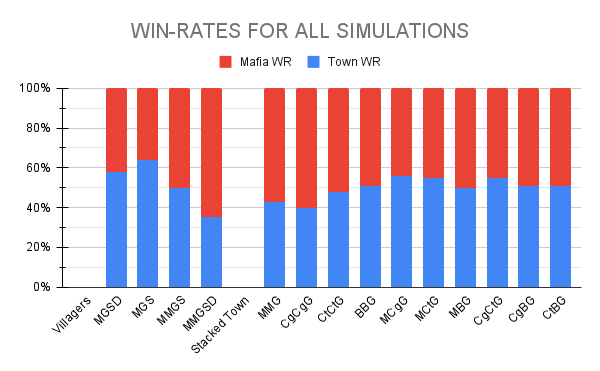
\includegraphics[width=1\linewidth]{figures/Winrates}
    \caption{\\Graph of the win-rate of various simulated game compositions.\\
        There were 10 players in each simulation.\\
        Each simulation was 100 games.
        Simulation names are related to team composition, based on role
        abbreviations in appendix \ref{app:A}.\\
        The first 4 runs labelled \textit{Villagers} means that all roles not
        mentioned in the abbreviation are replaced with villagers.\\
        The next runs labelled \textit{Powerful Town} means that all roles not
        mentioned in the abbreviation are replaced with	one of each town role.}
    \label{fig:VariousSimulations}
\end{figure}
\vspace{-5px}Based on this graph we can deduce that mafiosi and
consiglieri are more
impactful for the mafia than both consorts and blackmailers. But it also seems
that the varied team consisting of one mafioso, consigliere, and godfather,
performs marginally better than other configurations. \\
The results indicate that when playing against a powerful town, it is more
important for the mafia to be able to continually kill town members, and to be
able to quickly find the most powerful roles of the town, in order to eliminate
them, than it is to deny actions and communication to the town. \\
It would be interesting to see which of the non-killing mafia roles perform
best when they are on their own, and which composition of them perform best.
This type of game removes the mafias ability to kill during the night, while
they retain their knowledge of one another and their respective abilities to
gain information, limit nightly actions, and limit communicative actions. Below
are the results of such games:
\begin{figure}[H]
    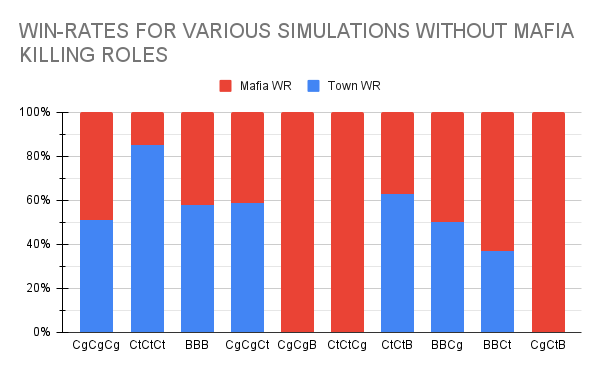
\includegraphics[width=1\linewidth]{figures/Winrates_NonKilling}
    \caption{\\Graph of the win-rate of various simulated game compositions
        with only non-killing mafia roles.\\
        There were 10 players in each simulation.\\
        Each simulation was 100 games.
        Simulation names are related to team composition, based on role
        abbreviations in appendix \ref{app:A}.\\
        All of the runs were against the previously explained powerful town.}
    \label{fig:VariousSimulationsNonKilling}
\end{figure}
\vspace{-5px} As seen on the above graph we can once again conclude that
consiglieri are more impactful than either consorts or blackmailers. This may
be due to their superior abilities in finding the sheriff, enabling them to 
collectively vote them out. It also seems that no mixed-combination of
non-killing mafia roles can compete with the pure-consiglieri team. 
